\subsection{Polynomial Decusping}
\begin{frame}[t]{Description}

\begin{itemize}
    \item Describe the method
\end{itemize}

\end{frame}

%%%%%%%%%%%%%%%%%%%%%%%%%%%%%%%%%%%%%%%%%%%%%%%%%%%%%%%%%%%%%%%%%%%%%%%%%%%%%%%%%

\begin{frame}[t]{Polynomials}
    
    show equations and pictures
    
\end{frame}

%%%%%%%%%%%%%%%%%%%%%%%%%%%%%%%%%%%%%%%%%%%%%%%%%%%%%%%%%%%%%%%%%%%%%%%%%%%%%%%%%

\subsection{Subplane Collision Probabilities}

\begin{frame}[t]{Subplane Decusping}
    
    \begin{itemize}
        \item Modifications made to subplane scheme \cite{Graham2017Improvementofthe2D/1DMethodUsingtheSub-PlaneScheme,Graham2017RodDecuspingTechniquesforthe2D/1DMethod} to treat axial effects of rod cusping
        \begin{itemize}
            \item Homogenization still uses MOC flux with axial shape factor, but 
            with heterogeneous rodded or unrodded cross sections
            \item Projection rehomogenizes cross sections in partially rodded nodes 
            after CMFD calculation
        \end{itemize}
        \begin{equation}\label{e:nTRACERdecusping}
        \overline{\Sigma_i} = \frac{\phi_{rad,i}^R \phi_{ax,i}^R \Sigma_i^R h^R + \phi_{rad,i}^U \phi_{ax,i}^U \Sigma_i^U h^U}{\phi_{rad,i}^R \phi_{ax,i}^R h^R + \phi_{rad,i}^U \phi_{ax,i}^U h^U} \nonumber
        \end{equation}
    \end{itemize}
    
\end{frame}

%%%%%%%%%%%%%%%%%%%%%%%%%%%%%%%%%%%%%%%%%%%%%%%%%%%%%%%%%%%%%%%%%%%%%%%%%%%%%%%%%

\begin{frame}[t]{Collision Probabilities Decusping}
    
    \begin{columns}
        \begin{column}{0.45\textwidth}
            \begin{itemize}
                \item Sub-plane modifications only capture axial effects
                \begin{itemize}
                    \item MOC uses homogenized cross section
                    \item Radial shape does not accurately reflect either region
                \end{itemize}
                \item 1D collision probabilities (CP) introduced to generate radial 
                shapes
                \begin{itemize}
                    \item Generates radial flux profile for rodded and unrodded region
                    \item Radial profiles used in CMFD homogenization
                    \item Very efficient calculation
                \end{itemize}
            \end{itemize}
        \end{column}
        \begin{column}{0.55\textwidth}
            \begin{figure}[h]
                \centering
                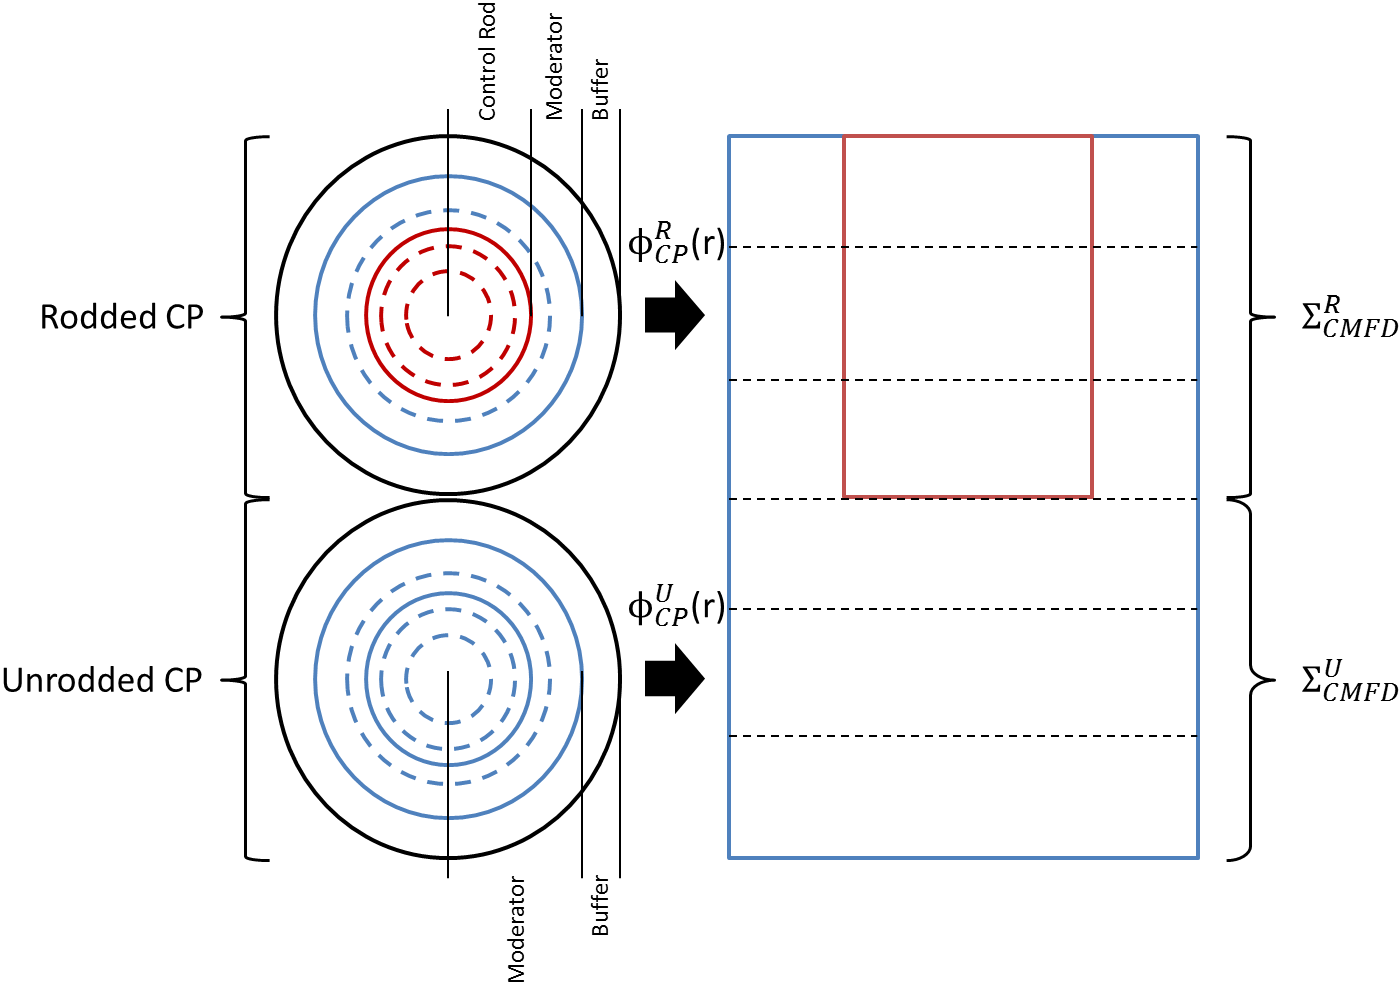
\includegraphics[width=\textwidth]{CPdecusp.png}
            \end{figure}
        \end{column}
    \end{columns}
    
\end{frame}

%%%%%%%%%%%%%%%%%%%%%%%%%%%%%%%%%%%%%%%%%%%%%%%%%%%%%%%%%%%%%%%%%%%%%%%%%%%%%%%%

\subsection{Subray Method of Characteristics}
\begin{frame}[t]{Description}

\begin{itemize}
    \item Motivate it
    \item Describe it
\end{itemize}

\end{frame}

%%%%%%%%%%%%%%%%%%%%%%%%%%%%%%%%%%%%%%%%%%%%%%%%%%%%%%%%%%%%%%%%%%%%%%%%%%%%%%%%

\begin{frame}
    
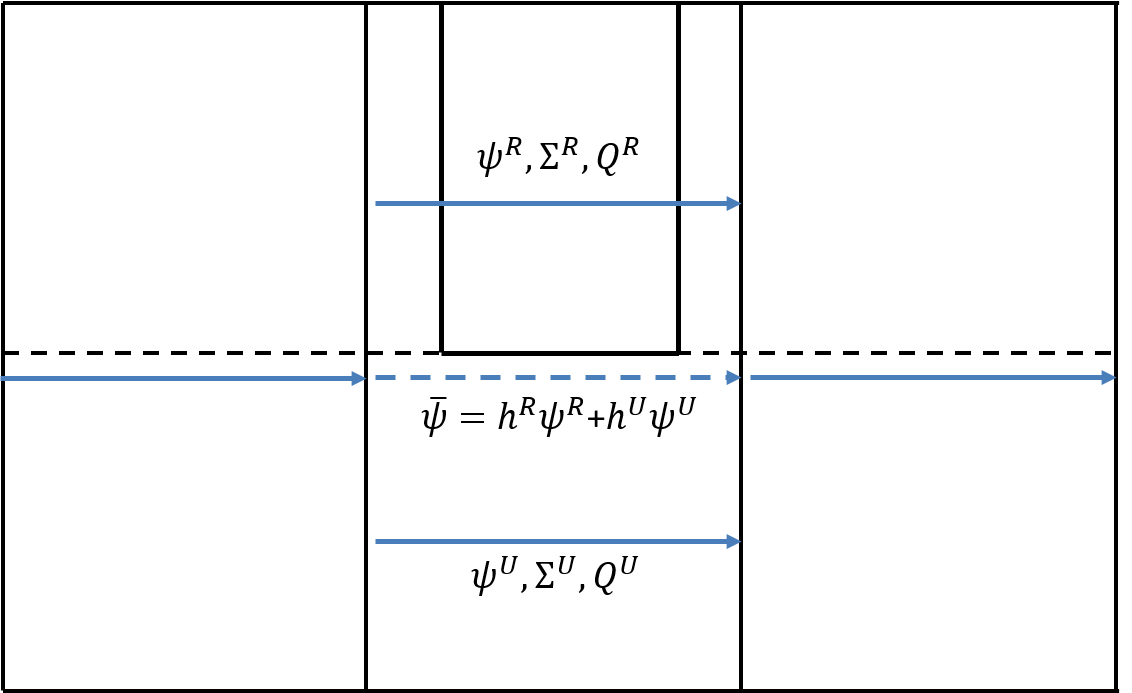
\includegraphics[width=0.8\textwidth]{sub-ray_illustration.png}

\end{frame}

%%%%%%%%%%%%%%%%%%%%%%%%%%%%%%%%%%%%%%%%%%%%%%%%%%%%%%%%%%%%%%%%%%%%%%%%%%%%%%%%

\begin{frame}[t]{2D/1D Modifications}
    
    \begin{itemize}
        \item Describe mods
    \end{itemize}

\end{frame}